\documentclass[main]{subfiles}
\begin{document}
\chapter{座標変換したセンサデータをプロットする}

これは講義資料「第4回 オドメトリと座標系」内の課題です。

\section{課題概要}
測域センサをつけたフリー状態(外力を受けて動く状態)の
ロボットを動かしてマッピングする。

ロボットを中心とした「方向」と「距離」の情報をもつ
極座標系のデータをセンサから受け取り、
ロボットを原点(0, 0)\footnote{(X座標, Y座標)}
とする直交座標系のデータ(FS座標系データ)に変換するだけの
プログラムが与えられる。
これをスタート地点を原点(0, 0)とする平面に関して唯一の値をとる
直交座標系のデータ(GL座標系データ)に変換する処理を記述してマッピングを行う。

\section{測域センサの概要}
測域センサには北陽電機株式会社のURG-04LXを使用する。
ロボットの前方に取り付けられたセンサはPCとUSB接続され、
PCとの通信にはSCIP2.0という通信プロトコルを利用する。

\section{解法}
\begin{figure}[H]
	\begin{minipage}{0.5\hsize}
		\setlength{\parindent}{1\Cwd}
		FS座標系もGL座標系も同一平面上の点の位置を定めるものなので、
		FS座標系で表現される点をGL座標系に変換するには、
		\textbf{現在地のGL座標}とスタート地点において$\theta = 0$と定義する
		\textbf{ロボットの傾き$\theta$}(rad)が必要となる。

		具体的な処理を明確にするためにプログラムを設計する前に右のような図を描いた。
		目的は、FS座標(Px, Py)で表現される赤い点をGL座標(glPx, glPy)に変換することだ。
		図ではXやYの表示が逆転しているものもあるが、軸に関しては正しく表示しているので
		パラメータの仮変数だと思って無視していただきたい。
	\end{minipage}
	\begin{minipage}{0.5\hsize}
		\begin{figure}[H]
			\centering
			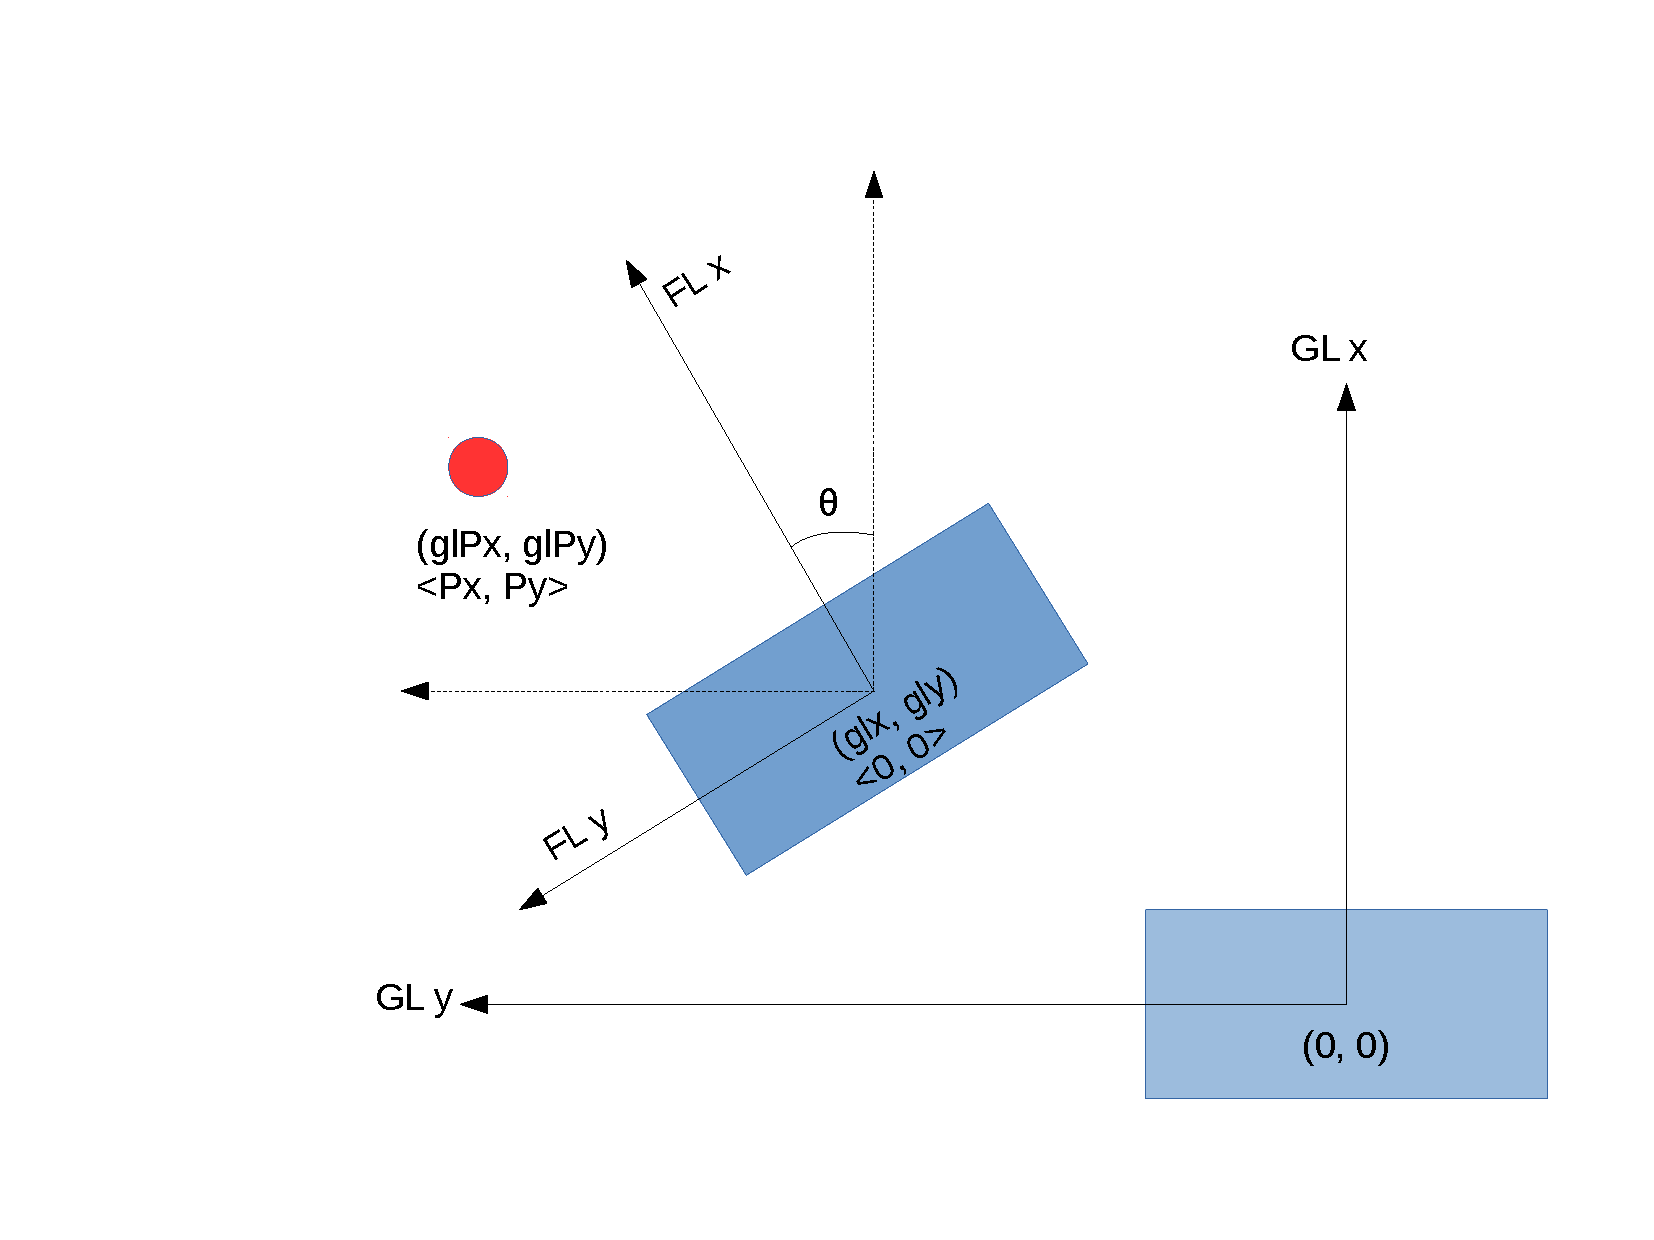
\includegraphics[width=8cm]{img/trans.pdf}
			\caption{FS座標系とGL座標系の関係}
		\end{figure}
	\end{minipage}
\end{figure}

まず現在のロボットの傾き\textit{pos\_theta\_gl}を用いて物体の座標を回転させる。
座標の回転といっても同一平面上の点の回転移動と同じであるから、
以下のような行列計算で求めることができる。
\[
	\left(
	\begin{array}{cc}
		x \\
		y
	\end{array}
	\right)
	=
	\left(
	\begin{array}{cc}
		cos(pos\_theta\_gl) & -sin(pos\_theta\_gl) \\
		sin(pos\_theta\_gl) & cos(pos\_theta\_gl)
	\end{array}
	\right)
	\left(
	\begin{array}{c}
		x\_fs \\
		y\_fs
	\end{array}
	\right)
\]

上記の記述でロボットの傾き$\theta $が0のときと同じ座標系に移すことができたが、
これでは原点がロボット中心になりマップを作ることができない。
ここで現在地のGL座標(pos\_x\_gl, pos\_y\_gl)を加算する。
これはGL座標の原点からFS座標の原点(ロボット中心)への単純な平行移動で実現される。
先の行列計算に合わせて記述すると以下のようになる。
\[
	\left(
	\begin{array}{cc}
		x\_gl \\
		y\_gl
	\end{array}
	\right)
	=
	\left(
	\begin{array}{c}
		pos\_x\_gl \\
		pos\_y\_gl
	\end{array}
	\right)
	+
	\left(
	\begin{array}{cc}
		cos(pos\_theta\_gl) & -sin(pos\_theta\_gl) \\
		sin(pos\_theta\_gl) & cos(pos\_theta\_gl)
	\end{array}
	\right)
	\left(
	\begin{array}{c}
		x\_fs \\
		y\_fs
	\end{array}
	\right)
\]

こうして得られる物体の座標はGL座標の原点を基準とした平面で唯一の座標である。

\section{結果}
実際にフリー状態のロボットを動かしてマッピングしてみる。

ノイズが目立つが正しくマッピングできている。

\section{考察}
座標系の変換がセンサをより強力なツールに変えた。
URGから送られるデータはロボットから
壁(単に光を反射するもの)までのベクトルに過ぎないが、
ロボットの位置情報を使った座標系の変換を行うことで、
世界中の壁を記録することができる。

第6章の最終課題では、これをさらに物体認識を行うツールへと強化する。
これにより単なる壁の記録のみならず、
同一物体を検出しオブジェクトとして記録できるようになる。

\end{document}
